% !TEX root = ../thesis.tex
\chapter{Einleitung}
\label{cha:intro}

Die Möglichkeiten einer dynamischen Speicherverwaltung haben sich in den meisten modernen Programmiersprachen etabliert\todo{JV: In welchen Sprachen nicht?}.
Die Vorteile, einen Teil des dynamischen Speichers -- oft auch als \textit{Heap} bezeichnet -- zur Laufzeit eines Programms anfordern zu können, sind unbestreitbar:
Speicherbereiche des Heaps dienen für Unterprogramme als Ablagemöglichkeit jenseits ihrer eigenen \textit{Stacks}, sodass abgelegte Inhalte nach Terminierung erhalten und für weitere Unterprogramme zugänglich bleiben.
Die Größe des angeforderten Speichers muss dabei nicht zur Übersetzungszeit bekannt sein, was die Realisierung dynamischer Datenstrukturen ermöglicht und die Überschreitung hartkodierter Speicherbereiche vermeidet\todo{s. JV}.

Für die konkrete Verwendung einer dynamischen Speicherverwaltung sind grundsätzlich zwei diametrale Ansätze denkbar:
Zum einen kann die Verantwortung für den korrekten Umgang mit dynamisch angefordertem Speicher gänzlich der Entwicklerin übertragen werden.
Dies ist in der Regel mit zusätzlichem Aufwand verbunden (vgl. \cite[S. 1f]{wilson1992}):
Speicheradressen müssen manuell verwaltet werden, Anweisungen zur Anforderung und Freigabe von Speicher müssen in den eigentlichen Code integriert werden und entsprechende Ausnahmefälle bei Fehlschlägen müssen ordnungsgemäß abgefangen werden.
Neben einer komplexer werdenden Codestruktur führt dies zu weiteren Fehlerquellen:
Die Freigabe noch benötigten Speichers führt zu so genannten \textit{hängenden Zeigern} (engl. \textit{dangling pointer}) -- Referenzen, die \textit{ins Leere zeigen} und in der Folge bestenfalls zu Programmabstürzen, schlimmstenfalls aber zu unerwartetem Verhalten und Datenverlust führen können.
Nicht freigegebener, aber nicht mehr benötigter Speicher kann wiederum zu \textit{Speicherlecks} (engl. \textit{memory leaks}) und -- bei hinreichend langer Laufzeit des Programms -- zu einer Ausschöpfung des Speichers führen.
\textit{Double frees}, bei denen Speicherbereiche doppelt freigegeben werden, sind eine weitere Ursache für unerwünschtes Programmverhalten.
Während die Anforderung von Speicher in der Regel unproblematisch ist, ist die Frage, wann und an welcher Stelle angeforderter Speicher wieder freigegeben werden kann, deutlich komplizierter, und fehlerhafte Verwendungen werden gegebenenfalls erst bei langfristiger Ausführung des Programms bemerkt.

Zum anderen existiert zur Vermeidung eben jener Schwierigkeiten der Ansatz, dem Compiler und der Laufzeitumgebung die adäquate Freigabe nicht mehr benötigten Speichers zu überlassen.
Zuständig hierfür ist dann ein Mechanismus, der gemeinhin als \textbf{Garbage Collection} (dt. \textit{Abfallentsorgung}) bezeichnet wird.
Eine Garbage Collection führt automatisch zu bestimmten Zeitpunkten -- etwa regelmäßig oder wenn akuter Speichermangel besteht -- eine Bereinigung des Speichers durch und gibt nicht mehr benötigte Speicherbereiche frei, ohne dass die Entwicklerin entsprechende Routinen in ihr Programm integrieren muss.
Nichtsdestoweniger wird dieser Komfortgewinn nicht ohne Nachteile erworben:
Wie jede Programmanweisung besitzt auch eine Garbage Collection einen gewissen Bedarf an Rechenzeit und Ressourcen, der sich negativ auf die Performance der eigentlichen Anwendung auswirken kann.
Vor allem in Anwendungen, die einen hohen Durchsatz erreichen wollen oder in denen Deadlines um jeden Preis eingehalten werden müssen, spielt die Auswahl eines geeigneten Garbage-Collection-Algorithmus eine signifikante Rolle\todo{JV: evtl. auf WCET in EmbSys hinweisen?}.

In dieser Arbeit werden wir gängige Ansätze zur Garbage Collection vorstellen und miteinander vergleichen.
Dabei soll auch ein Augenmerk auf Performance und Ressourcenbedarf gelegt sowie die Eignung in verschiedenen Anwendungsfällen beurteilt werden.
Im zweiten Teil der Arbeit wird der Entwurf und die Implementation einer Anwendung beschrieben, die die diskutierten Garbage-Collection-Algorithmen grafisch visualisiert und in einem vereinfachten Speichermodell simuliert.
Anhand dieser Anwendung soll die Arbeitsweise der Algorithmen veranschaulicht werden.

\section{Terminologie}
\label{sec:intro:terminologie}
Bevor wir genauer darauf eingehen, was unter einer Garbage Collection konkret verstanden wird, sollen zunächst die nötige Terminologie sowie ein Speichermodell eingeführt werden, das im Fortgang dieser Arbeit benutzt wird.
Dieses Speichermodell ist bewusst so abstrakt gehalten, dass es möglichst allgemeine Betrachtungen lösgelöst von gängigen Programmiersprachen, Laufzeitumgebungen und Betriebssystemen ermöglicht, auch wenn an einigen Stellen exemplarisch Bezüge zu diesen hergestellt werden.
Die eingeführten Begrifflichkeiten orientieren sich stark an der Terminologie aus \cite[Kap. 1]{jones-lins}.

\subsubsection*{Objekt}
Unter einem \textbf{Objekt} verstehen wir stets eine konkrete Instanz eines definierten Datentyps, beispielsweise eines \code{struct} in C oder einer Java-Klasse.
Ein Objekt besitzt eine festgelegte Anzahl von \textbf{Feldern}, die jeweils einen Wert eines festgelegten Datentyps -- etwa ein Integer oder eine Referenz auf ein anderes Objekt im hier definierten Sinne -- enthalten.
Der in dieser Arbeit verwendete Objektbegriff ist wesentlich allgemeiner gehalten als in der Objektorientierung üblich:
Auch einzelne Werte eines Basisdatentyps oder Arrays werden als Objekt aufgefasst, selbst wenn diese nicht Bestandteil eines im Programm definierten Datentyps sind.

Wir setzen ferner voraus, dass Objekte und ihre Felder \textit{typisiert} sind.
Das bedeutet, dass stets nachvollziehbar ist, aus welchen Feldern ein Objekt besteht von welchem Datentypen diese sind.
Insbesondere ist unterscheidbar, ob ein Feld eines Objekts eine Referenz enthält oder nicht.
Weiter nehmen wir an, dass jedes Objekt einen so genannten \textit{Header} besitzt.
Dies ist ein separates Feld, das Metainformationen aufnimmt, die für den Compiler und die Laufzeitumgebung, nicht aber aus Sicht des Entwicklers, zugänglich sind\todo{evtl genauer eingehen}.
Diverse vorgestellte Algorithmen werden diesen Bereich nutzen, um für die Speicherverwaltung relevante Informationen zu hinterlegen.

Den Zugriff auf das \code{i}-te Feld eines Objekts \code{a} notieren wir -- analog zur Syntax der Programmierspache C -- mit \code{a[i]}.
Ebenso bezeichnen wir mit \code{\&a} die Adresse eines Objekts und mit \code{*p} die Dereferenzierung eines Zeigers \code{p}.
Mit $\Pointers(\code{a})$ bezeichnen wir zudem die Menge aller Felder eines Objekts \code{a}, die eine Referenz enthalten können.

\subsubsection*{Heap}
Als \textbf{Heap} bezeichnen wir denjenigen Speicherbereich, in dem zur Laufzeit eines Programms Objekte in beliebiger Reihenfolge erzeugt und freigegeben werden können.
Der Heap besteht aus Blöcken einer festen Größe, auf die über eine Speicheradresse zugegriffen werden kann; ein \textit{Block} ist dabei die kleinste zuweisbare Speichermenge und kann die Zustände \textit{belegt} (bzw. \textit{zugewiesen}) oder \textit{frei} annehmen.
Sofern nichts anderes vereinbart ist, gehen wir davon aus, dass der Heap ein zusammenhängender linearer Speicherbereich ist.\footnote{Tatsächlich ist dies eine starke Vereinfachung. In der Praxis ist der Bereich des physikalischen Speichers, der von einer Anwendung verwendet wird, häufig fragmentiert und inhomogen. Die Speicherverwaltung eines Betriebssystems bildet diesen Bereich auf einen \textit{virtuellen Speicher} ab, der der Anwendung zu Verfügung gestellt wird und aus ihrer Sicht linear zusammenhängend ist. Für einen Überblick hierzu siehe etwa \cite[Kap. 3.3]{tanenbaum}.}

\todo[inline]{Grafik zu Heap und Objekten einfügen}

\subsubsection*{Allokator, Mutator und Kollektor}
Aufgabe des \textbf{Allokators}, der zur Laufzeitumgebung eines Programms gehört, ist zum einen die Zuweisung von Heapspeicher bei dynmaischer Instanziierung eines neuen Objektes und zum anderen die Freigabe von Objekten.
Der Allokator führt somit Buch über die belegten und freien Blöcke des Heaps.
Die genaue Realisierung dieser Mechanismen werden in dieser Arbeit weitestgehend außen vor gelassen, jedoch setzen wir in gewissen Situationen das Vorhandensein bestimmter Funktionalitäten voraus.
Beispielsweise verlangen wir, dass eine Prozedur \Method{new} zu Verfügung steht, die bei der Erzeugung eines neuen Objekts Speicher reserviert und die entsprechende Speicheradresse zurückgibt.
Die Funktionsweise von \Method{new} kann dabei vom verwendeten Garbage-Collection-Algorithmus abhängen (siehe Algorithmus~\ref{algo:new}).

\begin{algorithm}
\begin{algorithmic}[1]
	\State \MethodHead{new}():
	\State \quad \Var{adr} $\gets$ \Method{allocate}()		\Comment{Versuche Zuweisung von Speicher}
	\State \quad \IF \Var{adr} $=$ \Null		\Comment{Nicht genügend freier Speicher}
	\State \quad \quad \Method{collectGarbage}()	\Comment{Aufruf der Garbage Collection}
	\State \quad \quad \Var{adr} $\gets$ \Method{allocate}()	\Comment{Neuer Versuch}
	\State \quad \quad \IF \Var{adr} $=$ \Null
	\State \quad \quad \quad \Method{error}(\Var{"Nicht genügend Speicher"})
	\State \quad \Return \Var{adr}
\end{algorithmic}
\caption[Methode \Method{new} zur Erzeugung eines neuen Objekts]{Methode \Method{new} zur Erzeugung eines neuen Objekts. Die Garbage Collection wird hier bei Bedarf ausgelöst, wenn nicht genügend freier Speicher verfügbar ist.}
\label{algo:new}
\end{algorithm}

Nach Dijkstra et al. besteht ein Programm zudem aus zwei funktional unterscheidbaren Bestandteilen \cite[S. 967]{dijkstra1978}:
Der \textbf{Mutator} ist derjenige Thread (bzw. eine Menge von Threads), die den eigentlichen Programmcode ausführen.
Für uns sind dabei vor allem Programmanweisungen von Bedeutung, die in Feldern von Objekten vorhandene Referenzen manipulieren und somit ursächlich für die Entstehung von nicht mehr benötigten Objekten sind.
Im Gegensatz dazu ist es die Aufgabe des \textbf{Kollektors}, die nicht mehr benötigten Objekte zu identifizieren und ihre Freigabe zu veranlassen.
Der Kollektor ist demnach derjenige Thread (bzw. eine Menge von Threads), die einen Garbage-Collection-Algorithmus ausführen.

\section{Problemstellung}
\label{sec:intro:problem}
Nachdem die nötigen Grundbegriffe eingeführt wurden, können wir nun definieren, was wir unter einer Garbage Collection verstehen.
Anschließend folgt eine Spezifikation von Eigenschaften, die wir von einem Garbage-Collection-Algorithmus fordern.

\begin{mybox}
\begin{defn}[Lebendigkeit]
	\label{def:liveness}
	Ein Objekt heißt zu einem bestimmten Zeitpunkt im Programmablauf \textbf{lebendig}, wenn der Mutator im weiteren Programmablauf lesend oder schreibend auf dieses zugreift.
	Andernfalls bezeichnen wir das Objekt als \textit{nicht mehr benötigt}.
\end{defn}
\end{mybox}

\begin{mybox}
\begin{defn}[Garbage Collection]
	\label{def:gc}
	Eine Garbage Collection ist ein Algorithmus zur automatischen Wiederverwendung bereits genutzten Heapspeichers durch Identifikation und Freigabe von Objekten, die im weiteren Programmverlauf nicht mehr benötigt werden.
\end{defn}
\end{mybox}

Sobald der Mutator auf eine Objektinstanz im weiteren Programmverlauf nicht mehr zugreift -- weder lesend, noch schreibend -- ist ein Überschreiben des Objekts unproblematisch.
Demzufolge darf eine Garbage Collection die Freigabe des entsprechenden Speicherbereichs veranlassen, sobald eine Stelle im Programmcode erreicht wurde, ab der der Bezeichner eines Objekts (bzw. eine Referenz auf dieses Objekt) nicht mehr verwendet wird -- auch, wenn theoretisch noch darauf zugegriffen werden könnte.
Allerdings ist die Frage, ob dies der Fall ist oder nicht, nicht beantwortbar:

\begin{mybox}
\begin{satz}[Unentscheidbarkeit von Lebendigkeit]
	Es existiert kein Algorithmus, der die Lebendigkeit von Objekten entscheidet.
\end{satz}
\end{mybox}

\begin{proof}
	Dies ist ein Korollar aus der Unentscheidbarkeit des Halteproblems:
	Angenommen, es gäbe einen Algorithmus, der für ein beliebiges Programm entscheidet, ob Objekte zu einem bestimmten Zeitpunkt lebendig sind.
	Dieser müsste insbesondere entscheiden, dass der Teil eines Programms, in dem ein Objekt lebendig ist, terminiert.
	Ein solcher Algorithmus existiert jedoch nicht (vgl. \cite[Kap. 4.2]{sipser}).
\end{proof}

Aus diesem Grund betrachten wir eine schwächere Eigenschaft von Objekten: die Erreichbarkeit über Referenzen.
Dafür gehen wir von einer Menge \Roots von \textbf{Basisobjekten} (engl. \textit{root objects}) aus.
Diese sind dadurch gekennzeichnet, dass der Mutator unmittelbaren Zugriff auf sie hat, ohne dafür zunächst ihre Adresse aus den Feldern anderer Objekte beschaffen zu müssen.
Hierzu zählen zum Beispiel statische Objekte, deren Position im Speicher bereits zur Compilezeit bekannt ist, oder Objekte, die sich in \textit{stack frames}\todo{definieren} befinden.
Alle weiteren Objekte, die zur Laufzeit dynamisch erzeugt werden, gelten als erreichbar, wenn auf sie über eine Folge von Referenzen zugegriffen werden kann, wobei diese in den Feldern von Objekten gespeichert sind und die erste Referenz auf ein Basisobjekt verweist.
Einfacher ausgedrückt: Ein Objekt ist erreichbar, wenn der Mutator die Möglichkeit hat, mittelbar oder unmittelbar über Referenzen auf das Objekt zugreifen zu können.
Formal definieren wir diese Eigenschaft wie folgt:

\begin{mybox}
\begin{defn}[Erreichbarkeit]
	\label{def:erreichbar}
	Jedes Element der Menge $\Reach$ der erreichbaren Objekte ist durch endlich häufige Anwendung der folgenden beiden Regeln konstruiert:
	\begin{enumerate}[(1)]
		\item Ist $\code{a} \in \Roots$, so folgt $\code{a} \in \Reach$.
		\item Ist $\code{a} \in \Reach$, $\code{b}$ ein weiteres Objekt und existiert ein $i \in \NN$ mit $\code{*a[i]} = \code{b}$, so folgt $\code{b} \in \Reach$.
		In diesem Fall schreiben wir auch $\code{a} \rightarrow \code{b}$.
	\end{enumerate}
\end{defn}
\end{mybox}

Diese Definition garantiert zwar nicht, dass jedes erreichbare Objekt auch lebendig ist.
Davon ausgehend, dass unerreichbare Objekte auch nicht \textit{wiedergefunden} werden können, können wir jedoch mit Sicherheit sagen, dass unerreichbare Objekte nicht mehr verwendet werden und gefahrlos durch den Kollektor freigegeben werden dürfen.

Die Erreichbarkeit von Objekten lässt sich mithilfe eines sogenannten \textbf{Objektgraphen} visualisieren.
Jedes existierende Objekt korrespondiert dabei zu einem Knoten des Graphen.
Besitzt ein Objekt \code{a} in mindestens einem seiner Felder eine Referenz auf ein weiteres Objekt \code{b}, so wird dies durch eine gerichtete Kante zwischen den ensprechenden Knoten dargestellt.
Ein Objekt ist somit nicht erreichbar, wenn es im Objektgraphen keinen Pfad zu ihm gibt, der in einem Basisobjekt startet.
Objektgraphen werden uns im Rahmen dieser Arbeit bei der Veranschaulichng der vorgestellten Algorithmen dienlich sein.

	
\begin{mybox}
\begin{defn}[Objektgraph]
	Sei $O$ eine Menge von Objekten.
	Ein gerichteter Graph $G = (V,E)$ mit Knotenmenge $V$ und Kantenmenge $E \subseteq V \times V$ heißt Objektgraph, wenn eine bijektive Abbildung $\varphi \colon O \rightarrow V$ existiert, sodass für je zwei Objekte $\mathtt{a,b} \in O$ gilt:
	\[
		\mathtt{a} \rightarrow \mathtt{b} \quad \Leftrightarrow \quad (\varphi(\mathtt{a}),\varphi(\mathtt{b})) \in E.
	\]
\end{defn}
\end{mybox}

%\begin{mybox}
%\begin{defn}[Objektgraph]
%	Ein Objektgraph $G = (V,E)$ besteht aus einer Menge von Knoten $V$ und einer Menge von gerichteten Kanten $E \subseteq V \times V$, die wie folgt definiert sind:
%	\begin{enumerate}[(1)]
%		\item Ist \code{a} ein Objekt, so gilt $\code{a} \in V$.
%		\item Sind $\code{a}, \code{b} \in V$ und existiert ein $i \in \NN$ mit $\code{*a[i]} = \code{b}$, so ist $(\code{a},\code{b}) \in E$.
%	\end{enumerate}
%\end{defn}
%\end{mybox}

\begin{figure}[h]
	\centering
	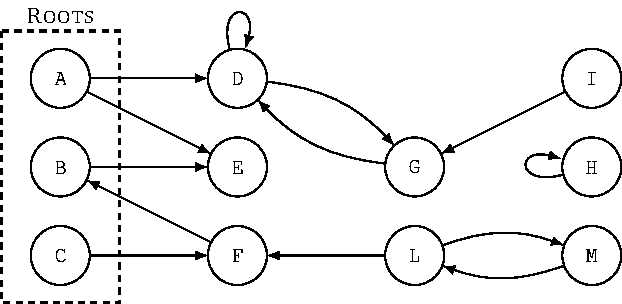
\includegraphics[keepaspectratio]{img/tikz/ch1-objgraph.pdf}
	\caption[Beispiel für einen Objektgraphen]{Beispiel für einen Objektgraphen. Die Objekte \code{A}, \code{B} und \code{C} sind Basisobjekte. Die Objekte \code{H}, \code{I}, \code{L} und \code{M} sind in dieser Kostellation nicht erreichbar.}
\end{figure}

An dieser Stelle formulieren wir ein Korrektheitskriterium für Garbage-Collection-Algorithmen.
Dieses besteht aus der Anforderung, dass keine noch benötigten Daten zerstört werden.

\begin{mybox}
\begin{defn}[Korrektheit für Garbage-Collection-Algorithmen]
	Ein Garbage-Collection-Algorithmus ist \textit{korrekt}, wenn er keine lebendigen Objekte freigibt.
\end{defn}
\end{mybox}

Gemäß Definition~\ref{def:erreichbar} ist es folglich hinreichend zu zeigen, dass nur nicht erreichbare Objekte freigegeben werden, um Korrektheit nachzuweisen.

Man kann an dieser Stelle fragen, warum wir nicht voraussetzen, dass die Ausführung eines Garbage-Collection-Algorithmus die Freigabe \textit{sämtlicher} nicht erreichbaren Objekte anfordert.
Tatsächlich werden wir sehen, dass es aus Performancegründen vorteilhaft sein kann, nur einen Teil des nicht mehr benötigten zugewiesenen Speichers zu bereinigen, um längere Wartezeiten zu vermeiden.
Ein solches Kriterium wäre daher zu restriktiv.